% Options for packages loaded elsewhere
\PassOptionsToPackage{unicode}{hyperref}
\PassOptionsToPackage{hyphens}{url}
%
\documentclass[
  ignorenonframetext,
]{beamer}
\usepackage{pgfpages}
\setbeamertemplate{caption}[numbered]
\setbeamertemplate{caption label separator}{: }
\setbeamercolor{caption name}{fg=normal text.fg}
\beamertemplatenavigationsymbolsempty
% Prevent slide breaks in the middle of a paragraph
\widowpenalties 1 10000
\raggedbottom
\setbeamertemplate{part page}{
  \centering
  \begin{beamercolorbox}[sep=16pt,center]{part title}
    \usebeamerfont{part title}\insertpart\par
  \end{beamercolorbox}
}
\setbeamertemplate{section page}{
  \centering
  \begin{beamercolorbox}[sep=12pt,center]{part title}
    \usebeamerfont{section title}\insertsection\par
  \end{beamercolorbox}
}
\setbeamertemplate{subsection page}{
  \centering
  \begin{beamercolorbox}[sep=8pt,center]{part title}
    \usebeamerfont{subsection title}\insertsubsection\par
  \end{beamercolorbox}
}
\AtBeginPart{
  \frame{\partpage}
}
\AtBeginSection{
  \ifbibliography
  \else
    \frame{\sectionpage}
  \fi
}
\AtBeginSubsection{
  \frame{\subsectionpage}
}

\usepackage{amsmath,amssymb}
\usepackage{iftex}
\ifPDFTeX
  \usepackage[T1]{fontenc}
  \usepackage[utf8]{inputenc}
  \usepackage{textcomp} % provide euro and other symbols
\else % if luatex or xetex
  \usepackage{unicode-math}
  \defaultfontfeatures{Scale=MatchLowercase}
  \defaultfontfeatures[\rmfamily]{Ligatures=TeX,Scale=1}
\fi
\usepackage{lmodern}
\ifPDFTeX\else  
    % xetex/luatex font selection
\fi
% Use upquote if available, for straight quotes in verbatim environments
\IfFileExists{upquote.sty}{\usepackage{upquote}}{}
\IfFileExists{microtype.sty}{% use microtype if available
  \usepackage[]{microtype}
  \UseMicrotypeSet[protrusion]{basicmath} % disable protrusion for tt fonts
}{}
\makeatletter
\@ifundefined{KOMAClassName}{% if non-KOMA class
  \IfFileExists{parskip.sty}{%
    \usepackage{parskip}
  }{% else
    \setlength{\parindent}{0pt}
    \setlength{\parskip}{6pt plus 2pt minus 1pt}}
}{% if KOMA class
  \KOMAoptions{parskip=half}}
\makeatother
\usepackage{xcolor}
\newif\ifbibliography
\setlength{\emergencystretch}{3em} % prevent overfull lines
\setcounter{secnumdepth}{-\maxdimen} % remove section numbering


\providecommand{\tightlist}{%
  \setlength{\itemsep}{0pt}\setlength{\parskip}{0pt}}\usepackage{longtable,booktabs,array}
\usepackage{calc} % for calculating minipage widths
\usepackage{caption}
% Make caption package work with longtable
\makeatletter
\def\fnum@table{\tablename~\thetable}
\makeatother
\usepackage{graphicx}
\makeatletter
\def\maxwidth{\ifdim\Gin@nat@width>\linewidth\linewidth\else\Gin@nat@width\fi}
\def\maxheight{\ifdim\Gin@nat@height>\textheight\textheight\else\Gin@nat@height\fi}
\makeatother
% Scale images if necessary, so that they will not overflow the page
% margins by default, and it is still possible to overwrite the defaults
% using explicit options in \includegraphics[width, height, ...]{}
\setkeys{Gin}{width=\maxwidth,height=\maxheight,keepaspectratio}
% Set default figure placement to htbp
\makeatletter
\def\fps@figure{htbp}
\makeatother

\makeatletter
\makeatother
\makeatletter
\makeatother
\makeatletter
\@ifpackageloaded{caption}{}{\usepackage{caption}}
\AtBeginDocument{%
\ifdefined\contentsname
  \renewcommand*\contentsname{Table of contents}
\else
  \newcommand\contentsname{Table of contents}
\fi
\ifdefined\listfigurename
  \renewcommand*\listfigurename{List of Figures}
\else
  \newcommand\listfigurename{List of Figures}
\fi
\ifdefined\listtablename
  \renewcommand*\listtablename{List of Tables}
\else
  \newcommand\listtablename{List of Tables}
\fi
\ifdefined\figurename
  \renewcommand*\figurename{Figure}
\else
  \newcommand\figurename{Figure}
\fi
\ifdefined\tablename
  \renewcommand*\tablename{Table}
\else
  \newcommand\tablename{Table}
\fi
}
\@ifpackageloaded{float}{}{\usepackage{float}}
\floatstyle{ruled}
\@ifundefined{c@chapter}{\newfloat{codelisting}{h}{lop}}{\newfloat{codelisting}{h}{lop}[chapter]}
\floatname{codelisting}{Listing}
\newcommand*\listoflistings{\listof{codelisting}{List of Listings}}
\makeatother
\makeatletter
\@ifpackageloaded{caption}{}{\usepackage{caption}}
\@ifpackageloaded{subcaption}{}{\usepackage{subcaption}}
\makeatother
\makeatletter
\@ifpackageloaded{tcolorbox}{}{\usepackage[skins,breakable]{tcolorbox}}
\makeatother
\makeatletter
\@ifundefined{shadecolor}{\definecolor{shadecolor}{rgb}{.97, .97, .97}}
\makeatother
\makeatletter
\makeatother
\makeatletter
\makeatother
\ifLuaTeX
  \usepackage{selnolig}  % disable illegal ligatures
\fi
\IfFileExists{bookmark.sty}{\usepackage{bookmark}}{\usepackage{hyperref}}
\IfFileExists{xurl.sty}{\usepackage{xurl}}{} % add URL line breaks if available
\urlstyle{same} % disable monospaced font for URLs
\hypersetup{
  pdftitle={The least squared Methods},
  hidelinks,
  pdfcreator={LaTeX via pandoc}}

\title{The least squared Methods}
\author{}
\date{}

\begin{document}
\frame{\titlepage}
\ifdefined\Shaded\renewenvironment{Shaded}{\begin{tcolorbox}[frame hidden, breakable, sharp corners, enhanced, borderline west={3pt}{0pt}{shadecolor}, interior hidden, boxrule=0pt]}{\end{tcolorbox}}\fi

\begin{frame}{Simple Linear Model}
\protect\hypertarget{simple-linear-model}{}
\begin{itemize}
\tightlist
\item
  Given the data
\end{itemize}

\begin{longtable}[]{@{}ll@{}}
\toprule\noalign{}
\(x\) & \(y\) \\
\midrule\noalign{}
\endhead
1 & 1.1 \\
2 & 1.8 \\
3 & 2.7 \\
4 & 4.5 \\
\bottomrule\noalign{}
\end{longtable}
\end{frame}

\begin{frame}{Scatter plot}
\protect\hypertarget{scatter-plot}{}
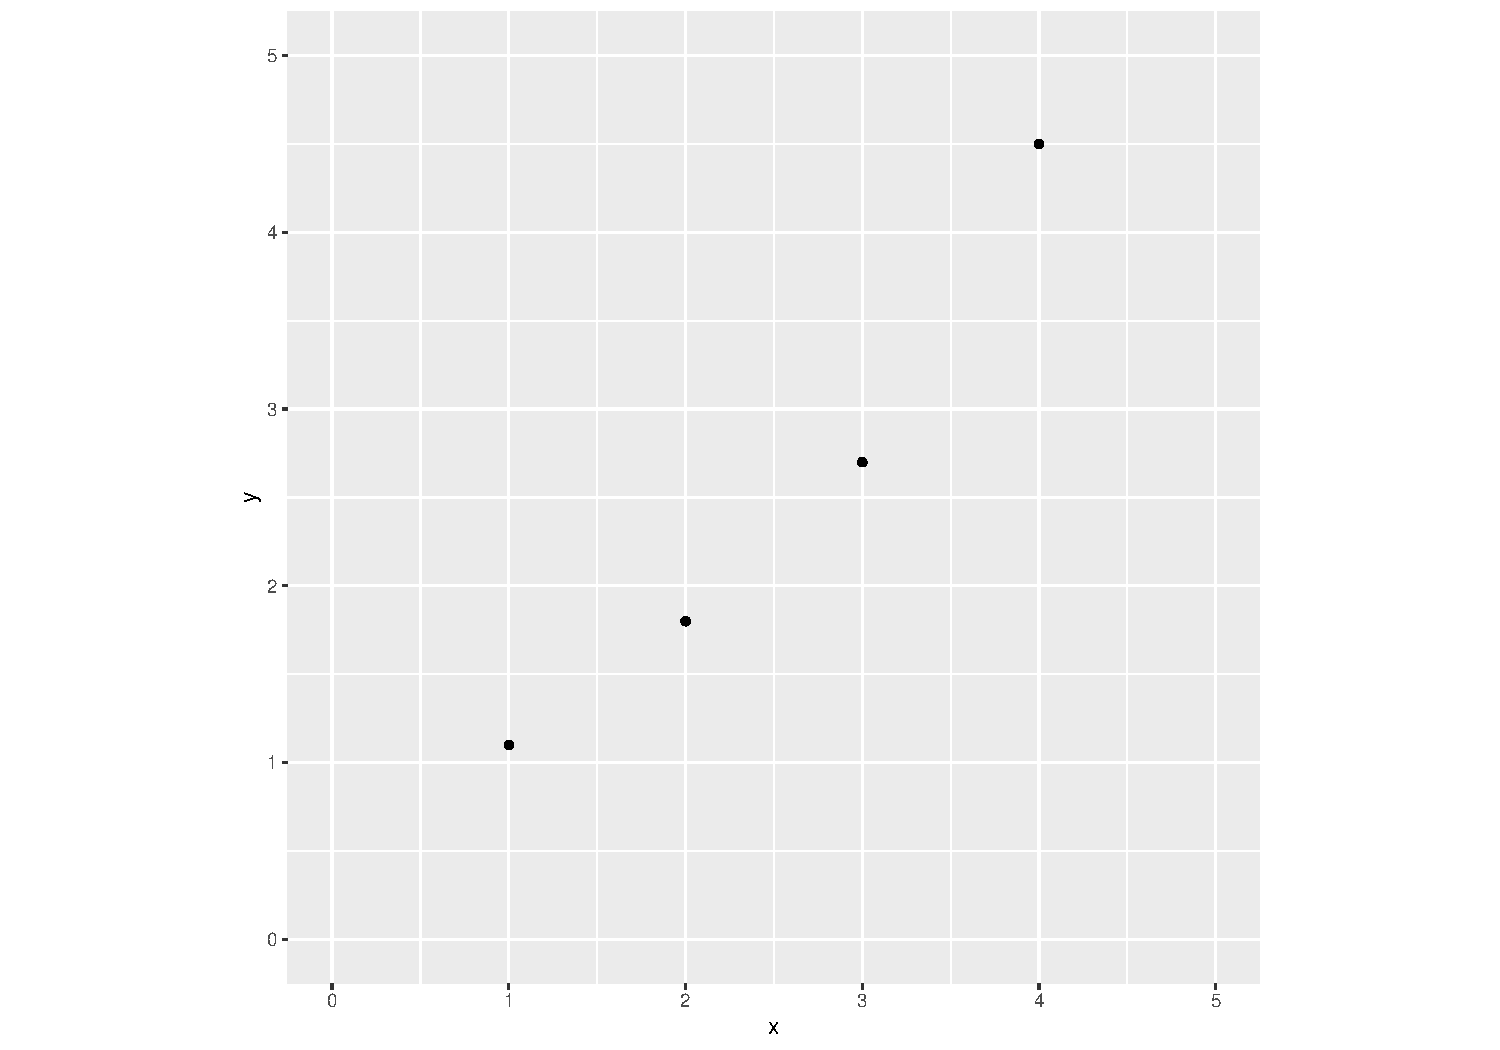
\includegraphics{1_files/figure-beamer/unnamed-chunk-2-1.pdf}
\end{frame}

\begin{frame}{Which line is closer to the points?}
\protect\hypertarget{which-line-is-closer-to-the-points}{}
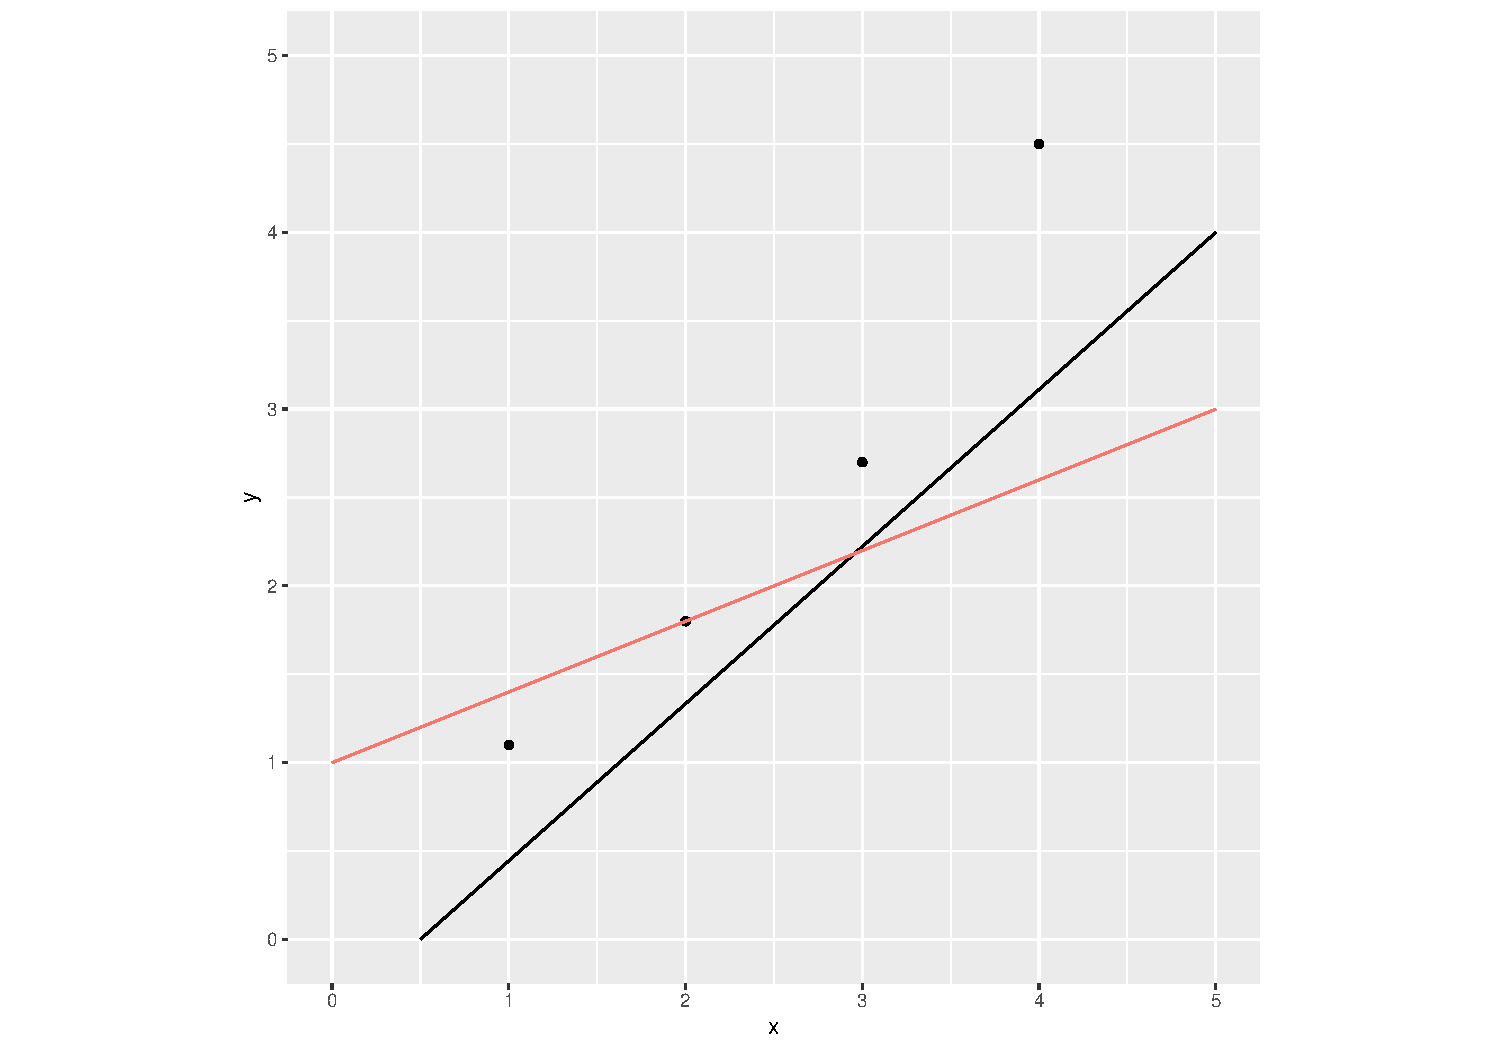
\includegraphics{1_files/figure-beamer/unnamed-chunk-3-1.pdf}
\end{frame}

\begin{frame}{Squared Distance between a line and points}
\protect\hypertarget{squared-distance-between-a-line-and-points}{}
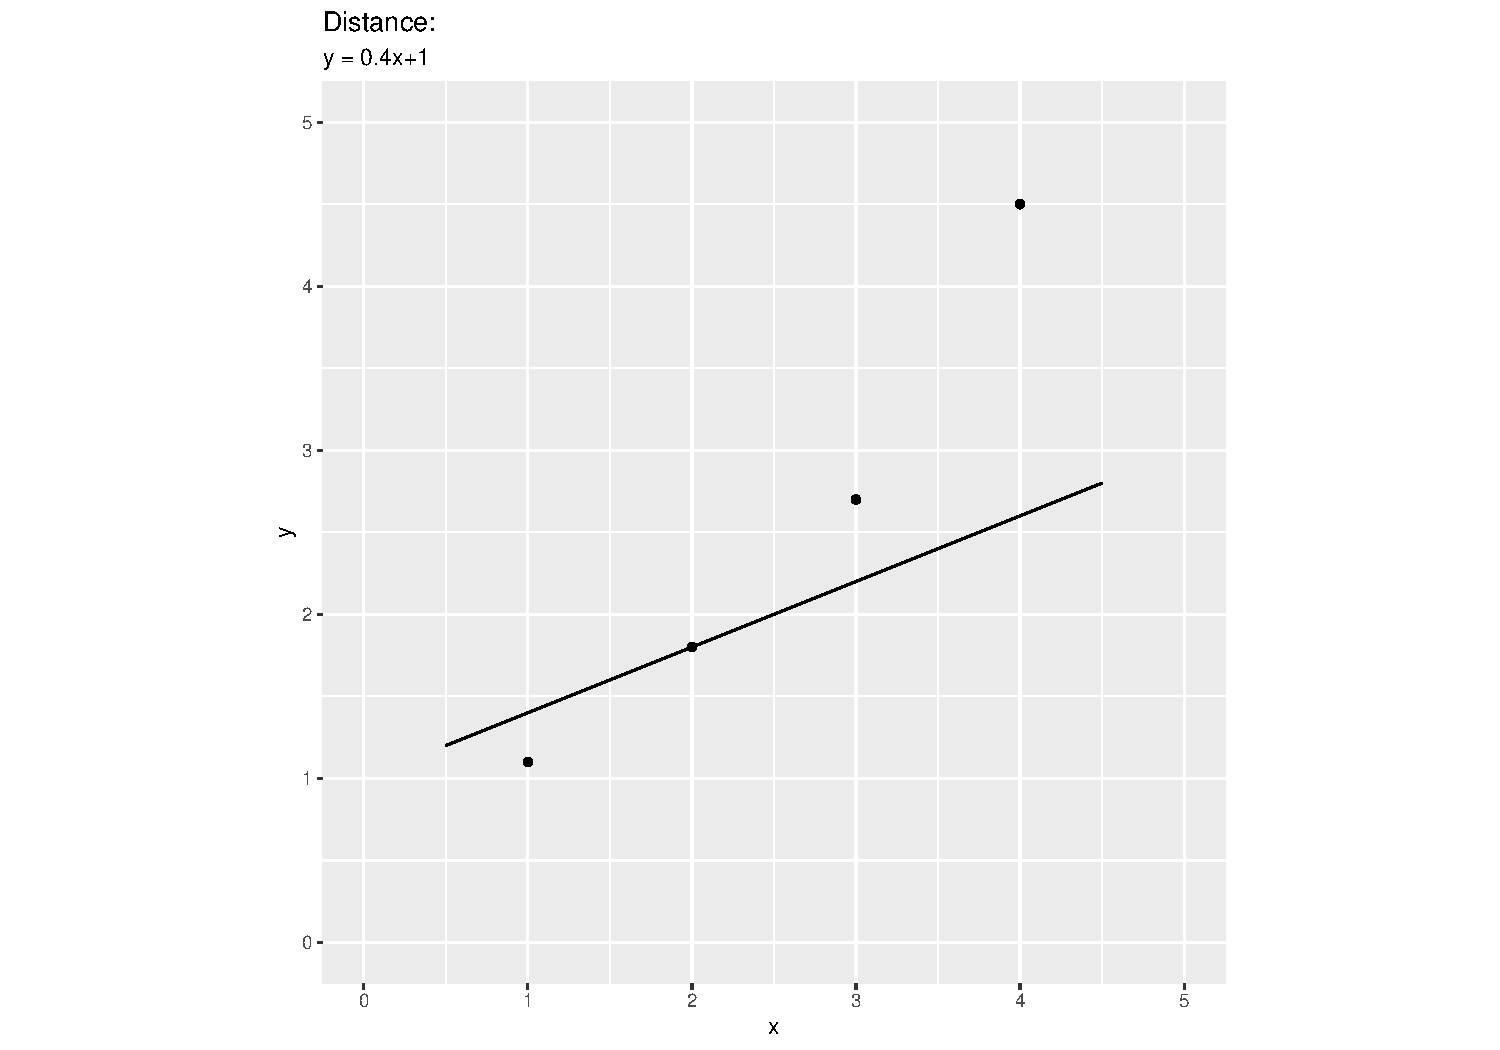
\includegraphics{1_files/figure-beamer/unnamed-chunk-4-1.pdf}
\end{frame}

\begin{frame}{Squared Distance between a line and points}
\protect\hypertarget{squared-distance-between-a-line-and-points-1}{}
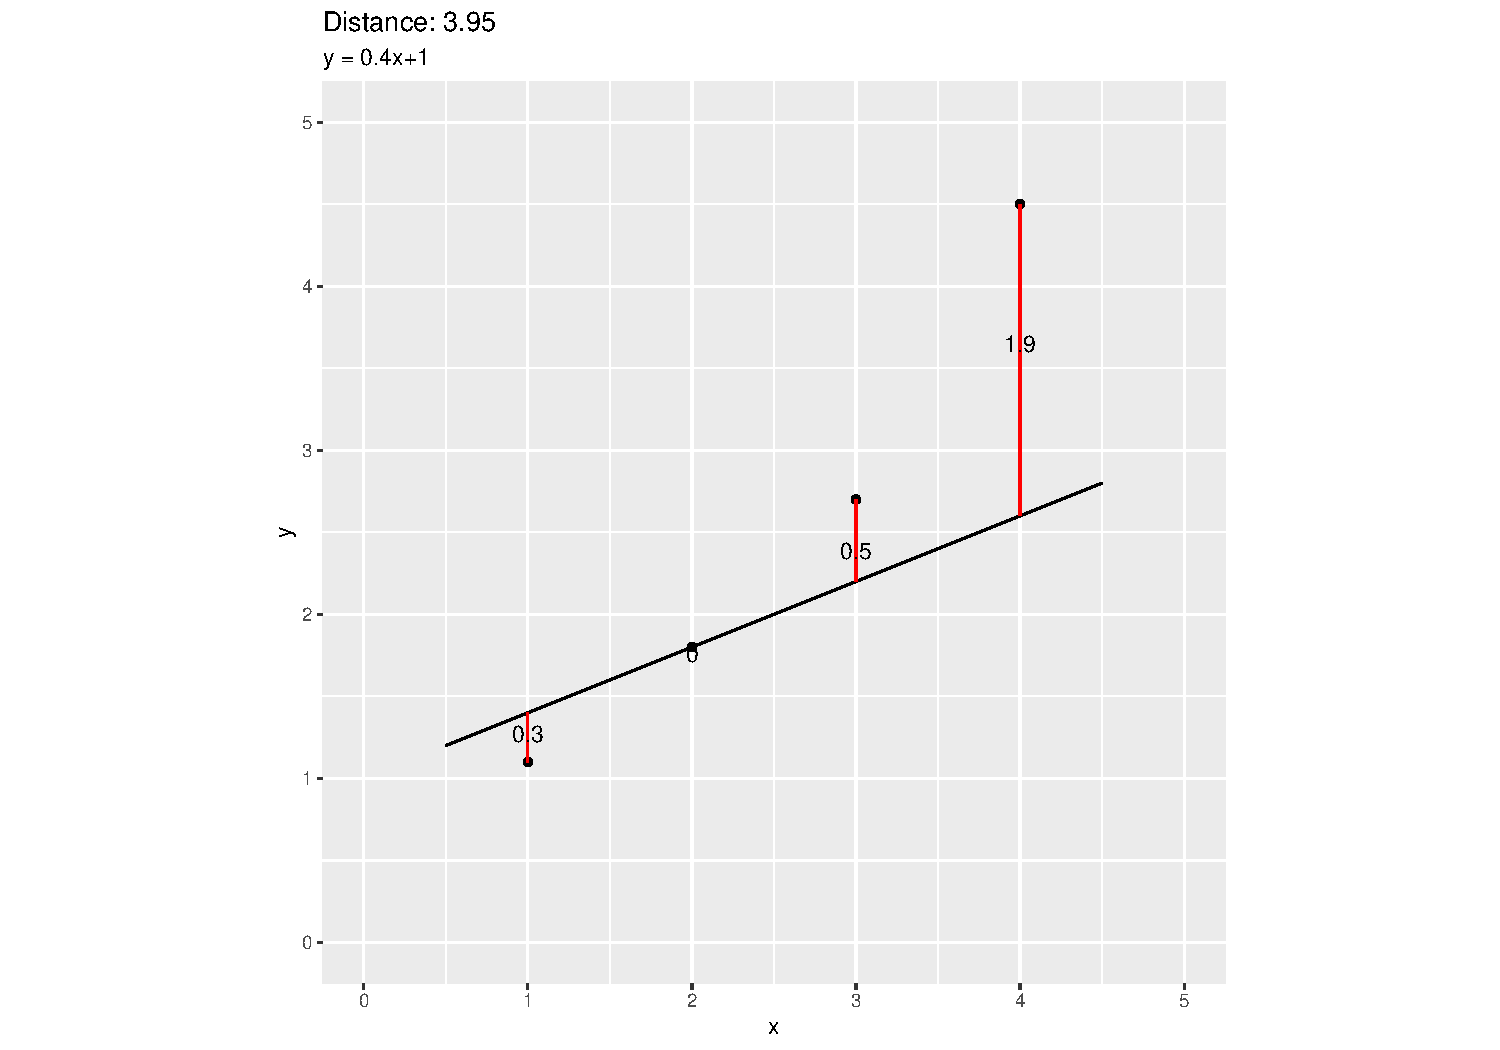
\includegraphics{1_files/figure-beamer/unnamed-chunk-5-1.pdf}
\end{frame}

\begin{frame}{Squared Distance between a line and points}
\protect\hypertarget{squared-distance-between-a-line-and-points-2}{}
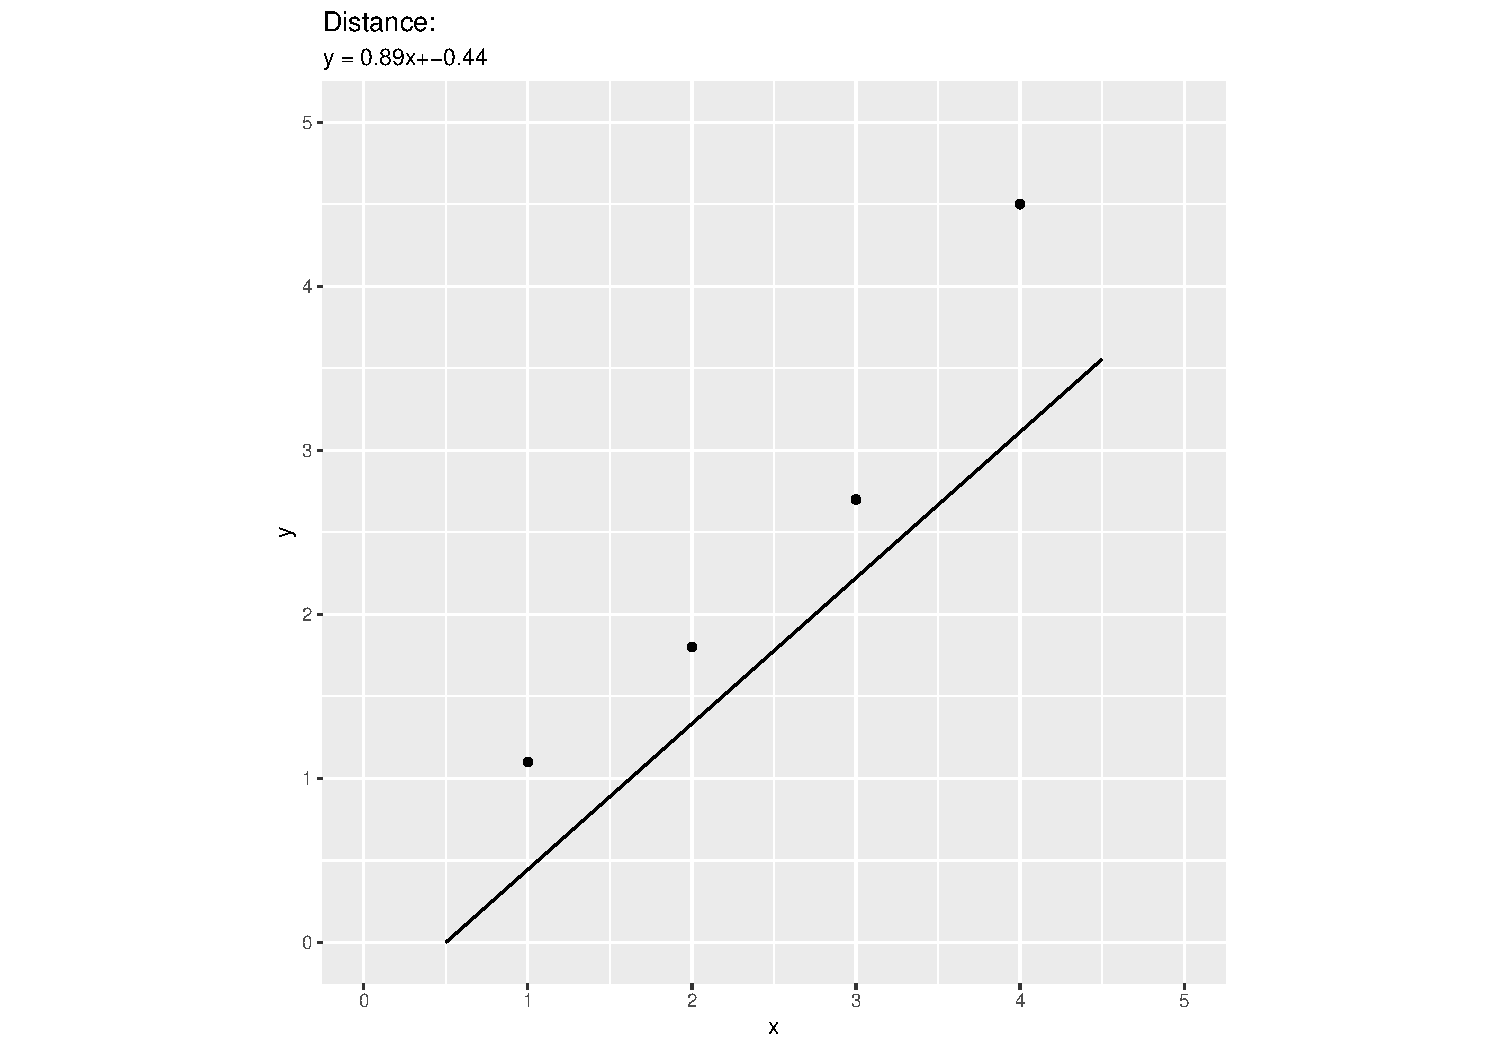
\includegraphics{1_files/figure-beamer/unnamed-chunk-6-1.pdf}
\end{frame}

\begin{frame}{Squared Distance between a line and points}
\protect\hypertarget{squared-distance-between-a-line-and-points-3}{}
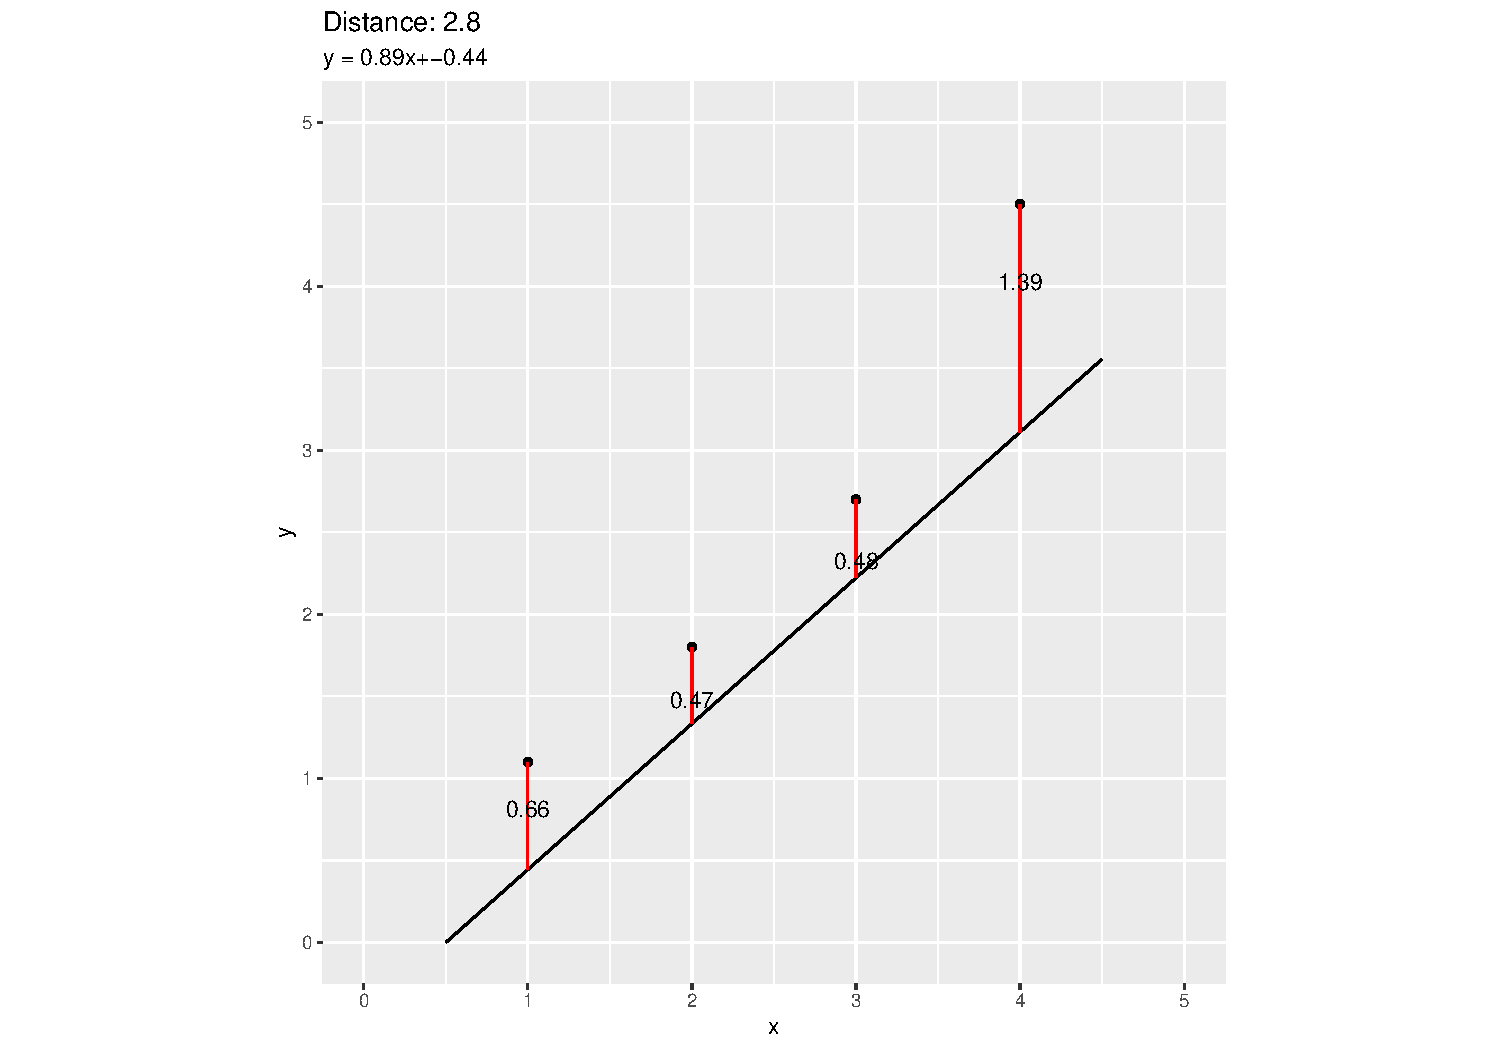
\includegraphics{1_files/figure-beamer/unnamed-chunk-7-1.pdf}
\end{frame}

\begin{frame}[fragile]{What is the closest line to the points?}
\protect\hypertarget{what-is-the-closest-line-to-the-points}{}
\begin{itemize}
\item
  The least squared methods give us the formula for the \texttt{closest}
  line:
\item
  \(y = \hat{\beta_1}x+\hat{\beta_0}\)
\item
  \(\hat{\beta_{1}} = \frac{\sum_{i=1}^{n}{(x_i-\bar{x})(y_i-\bar{y})}}{\sum_{i=1}^{n}(x_i-\bar{x})^2} = \frac{S_{xy}}{S_{xx}}\)
\item
  \(\hat{\beta_{0}} = \bar{y} - \hat{\beta_{1}}\bar{x}\)
\item
  This line is also called the best fitted line
\end{itemize}
\end{frame}

\begin{frame}{Calculation}
\protect\hypertarget{calculation}{}
\begin{longtable}[]{@{}ll@{}}
\toprule\noalign{}
\(x\) & \(y\) \\
\midrule\noalign{}
\endhead
1 & 1.1 \\
2 & 1.8 \\
3 & 2.7 \\
4 & 4.5 \\
\bottomrule\noalign{}
\end{longtable}
\end{frame}

\begin{frame}{Calculation}
\protect\hypertarget{calculation-1}{}
\begin{longtable}[]{@{}ccccc@{}}
\toprule\noalign{}
& \(x\) & \(y\) & \(xy\) & \(x^2\) \\
\midrule\noalign{}
\endhead
& 1 & 1.1 & & \\
& 2 & 1.8 & & \\
& 3 & 2.7 & & \\
& 4 & 4.5 & & \\
\(\sum\) & & & & \\
\bottomrule\noalign{}
\end{longtable}
\end{frame}

\begin{frame}{Calculation}
\protect\hypertarget{calculation-2}{}
\begin{longtable}[]{@{}ccccc@{}}
\toprule\noalign{}
& \(x\) & \(y\) & \(xy\) & \(x^2\) \\
\midrule\noalign{}
\endhead
& 1 & 1.1 & & \\
& 2 & 1.8 & & \\
& 3 & 2.7 & & \\
& 4 & 4.5 & & \\
\(\sum\) & & & & \\
\bottomrule\noalign{}
\end{longtable}

\begin{itemize}
\tightlist
\item
  \(\bar{x} = \frac{1+2+3+4}{4} = 2.5\)
\item
  \(\bar{y} = \frac{1.1+1.8+2.4+4.5}{4} = 2.525\)
\end{itemize}
\end{frame}

\begin{frame}{Calculation}
\protect\hypertarget{calculation-3}{}
\begin{longtable}[]{@{}ccccc@{}}
\toprule\noalign{}
& \(x\) & \(y\) & \(xy\) & \(x^2\) \\
\midrule\noalign{}
\endhead
& 1 & 1.1 & 1.1 & 1 \\
& 2 & 1.8 & 3.6 & 4 \\
& 3 & 2.7 & 8.1 & 9 \\
& 4 & 4.5 & 18 & 16 \\
\(\sum\) & & & 30.8 & 30 \\
\bottomrule\noalign{}
\end{longtable}

\begin{itemize}
\item
  \(\hat{\beta_1} = \frac{\sum xy -n\bar{x}\bar{y}}{\sum x^2 - n\bar{x}^2} = 1.11\)
\item
  \(\hat{\beta_0} = \bar{y} - \hat{\beta_{1}}\bar{x} = -0.25\)
\end{itemize}
\end{frame}

\begin{frame}{Graph}
\protect\hypertarget{graph}{}
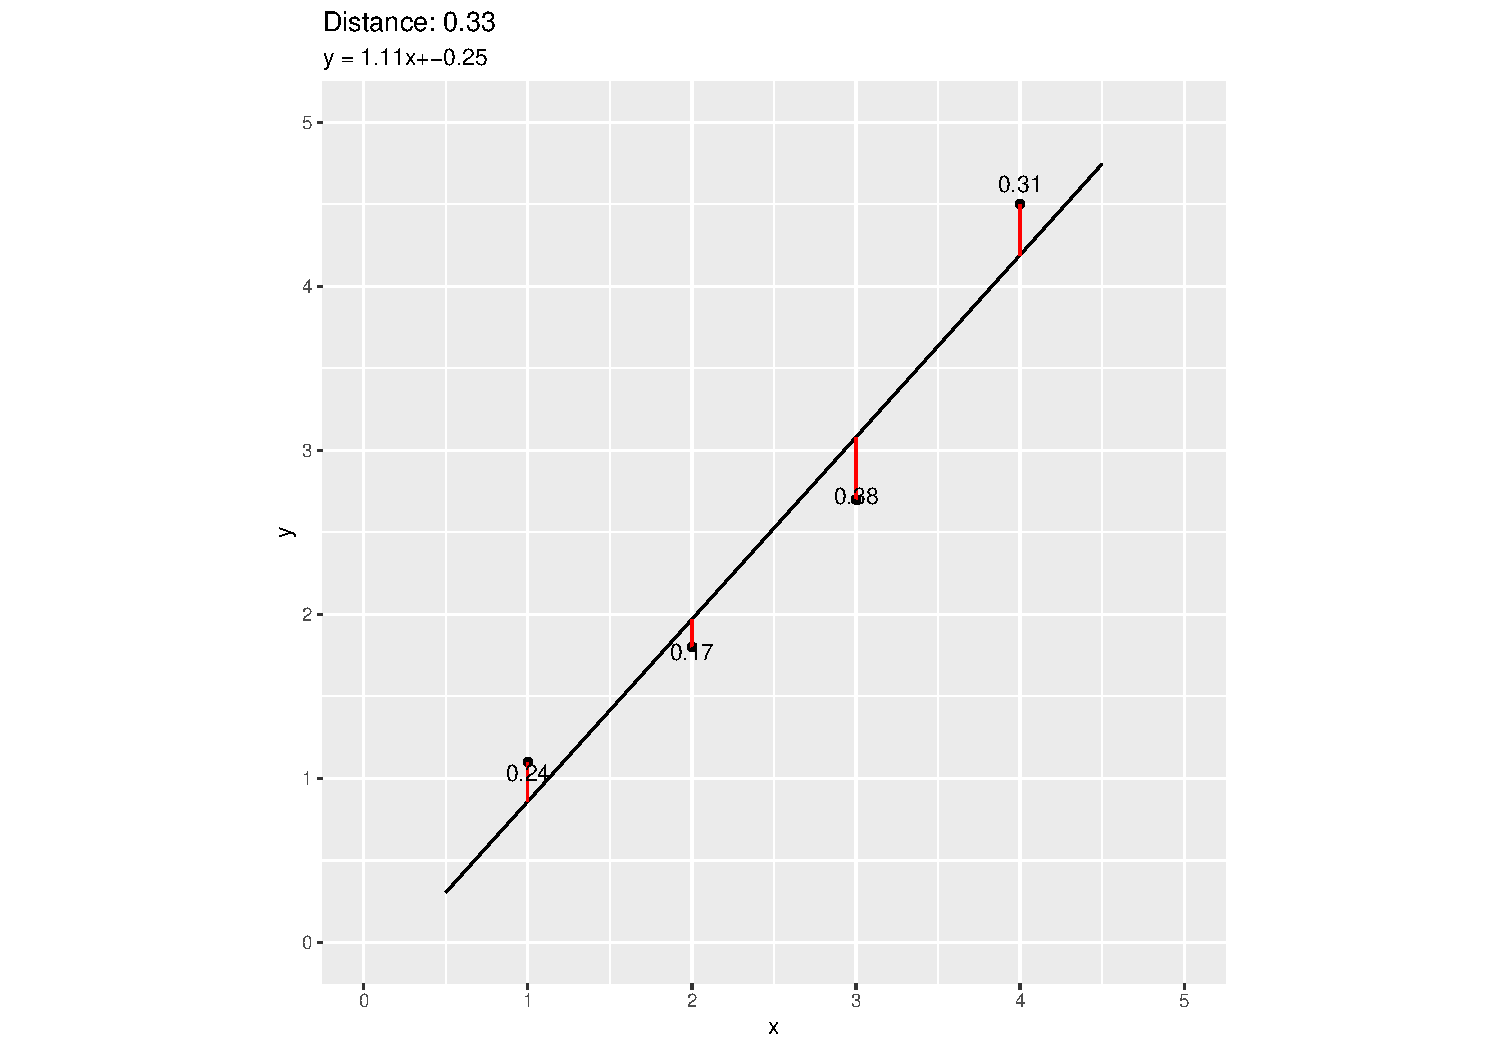
\includegraphics{1_files/figure-beamer/unnamed-chunk-8-1.pdf}
\end{frame}

\begin{frame}{Some other lines}
\protect\hypertarget{some-other-lines}{}
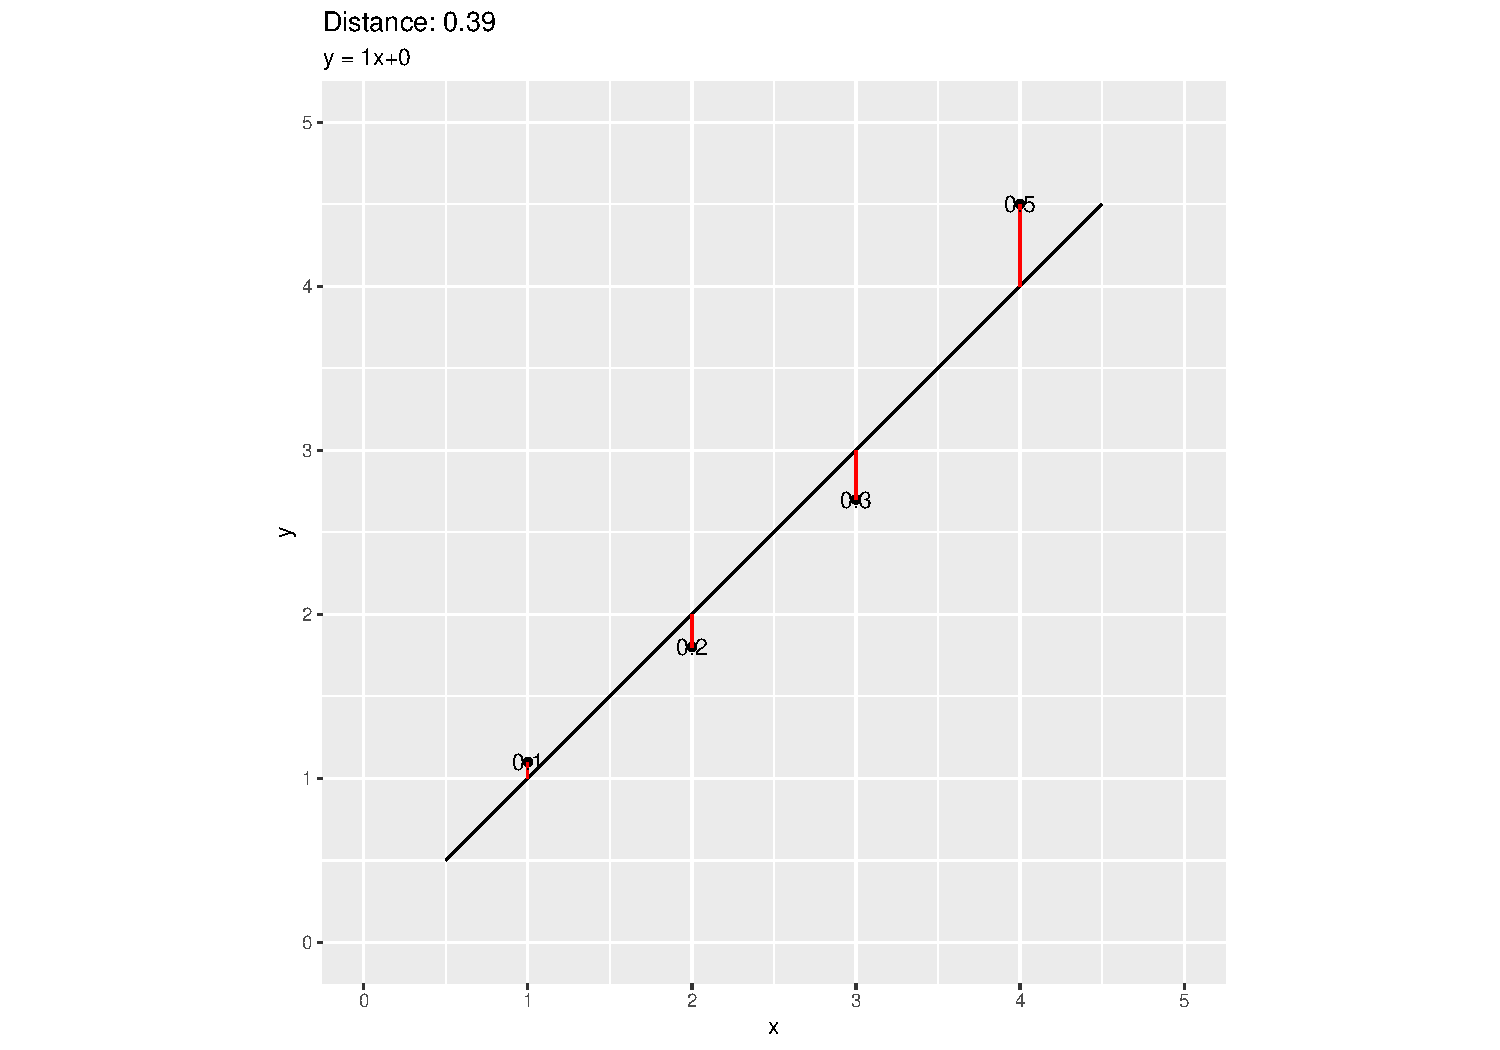
\includegraphics{1_files/figure-beamer/unnamed-chunk-9-1.pdf}
\end{frame}

\begin{frame}{Some other lines}
\protect\hypertarget{some-other-lines-1}{}
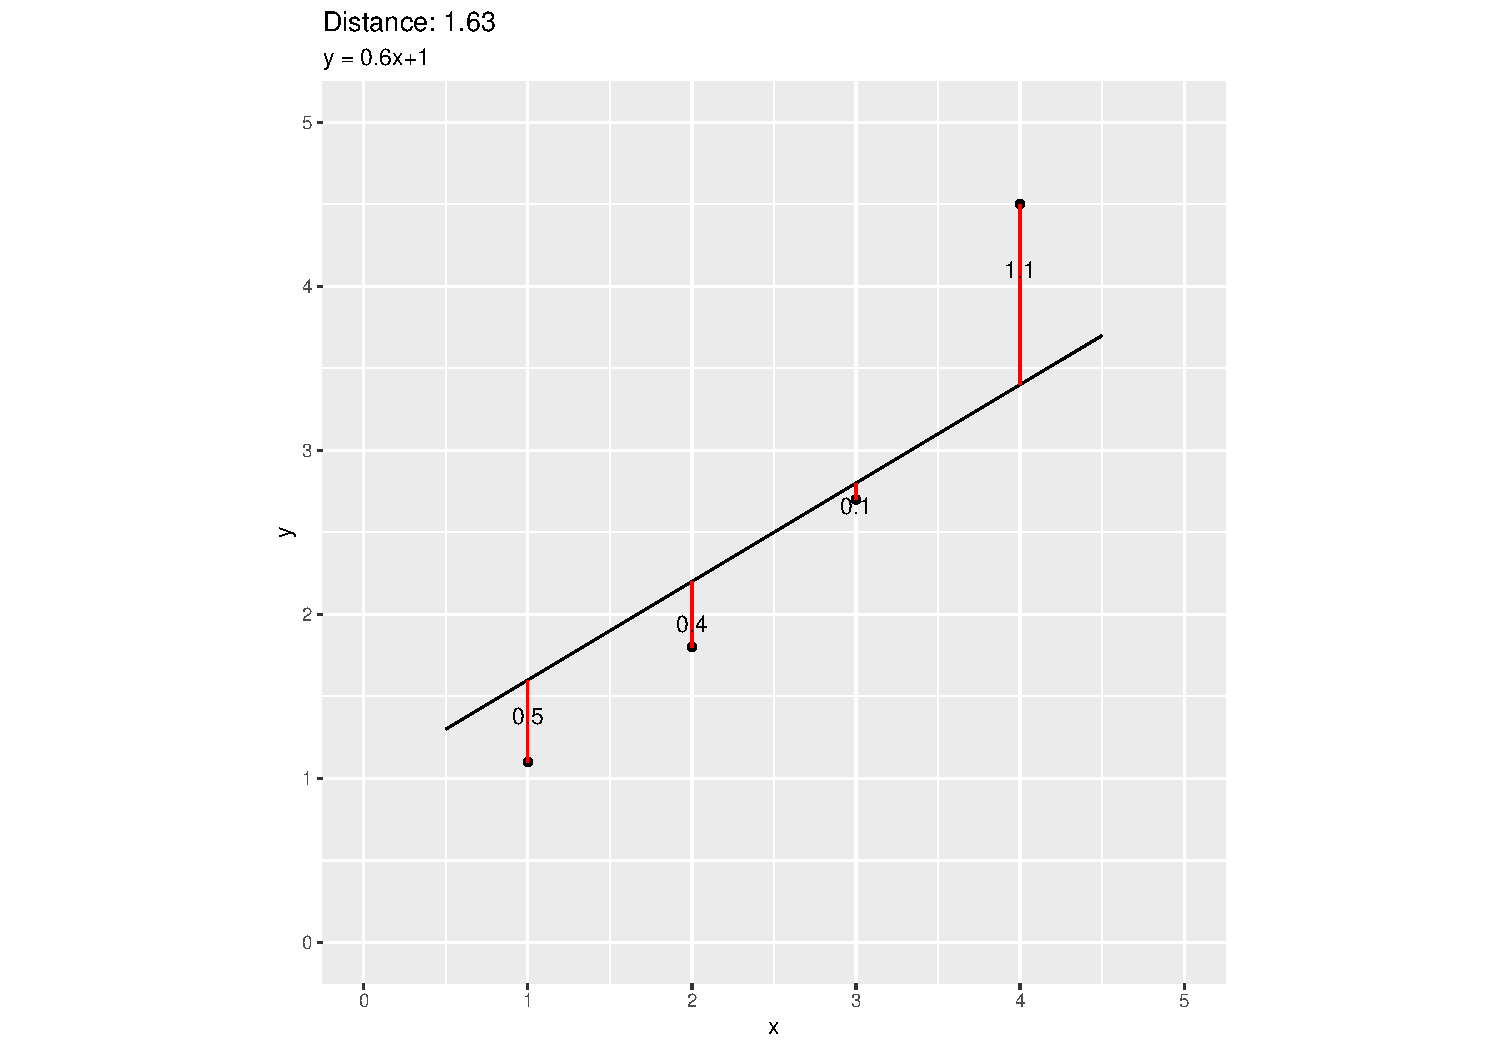
\includegraphics{1_files/figure-beamer/unnamed-chunk-10-1.pdf}
\end{frame}

\begin{frame}{Some other lines}
\protect\hypertarget{some-other-lines-2}{}
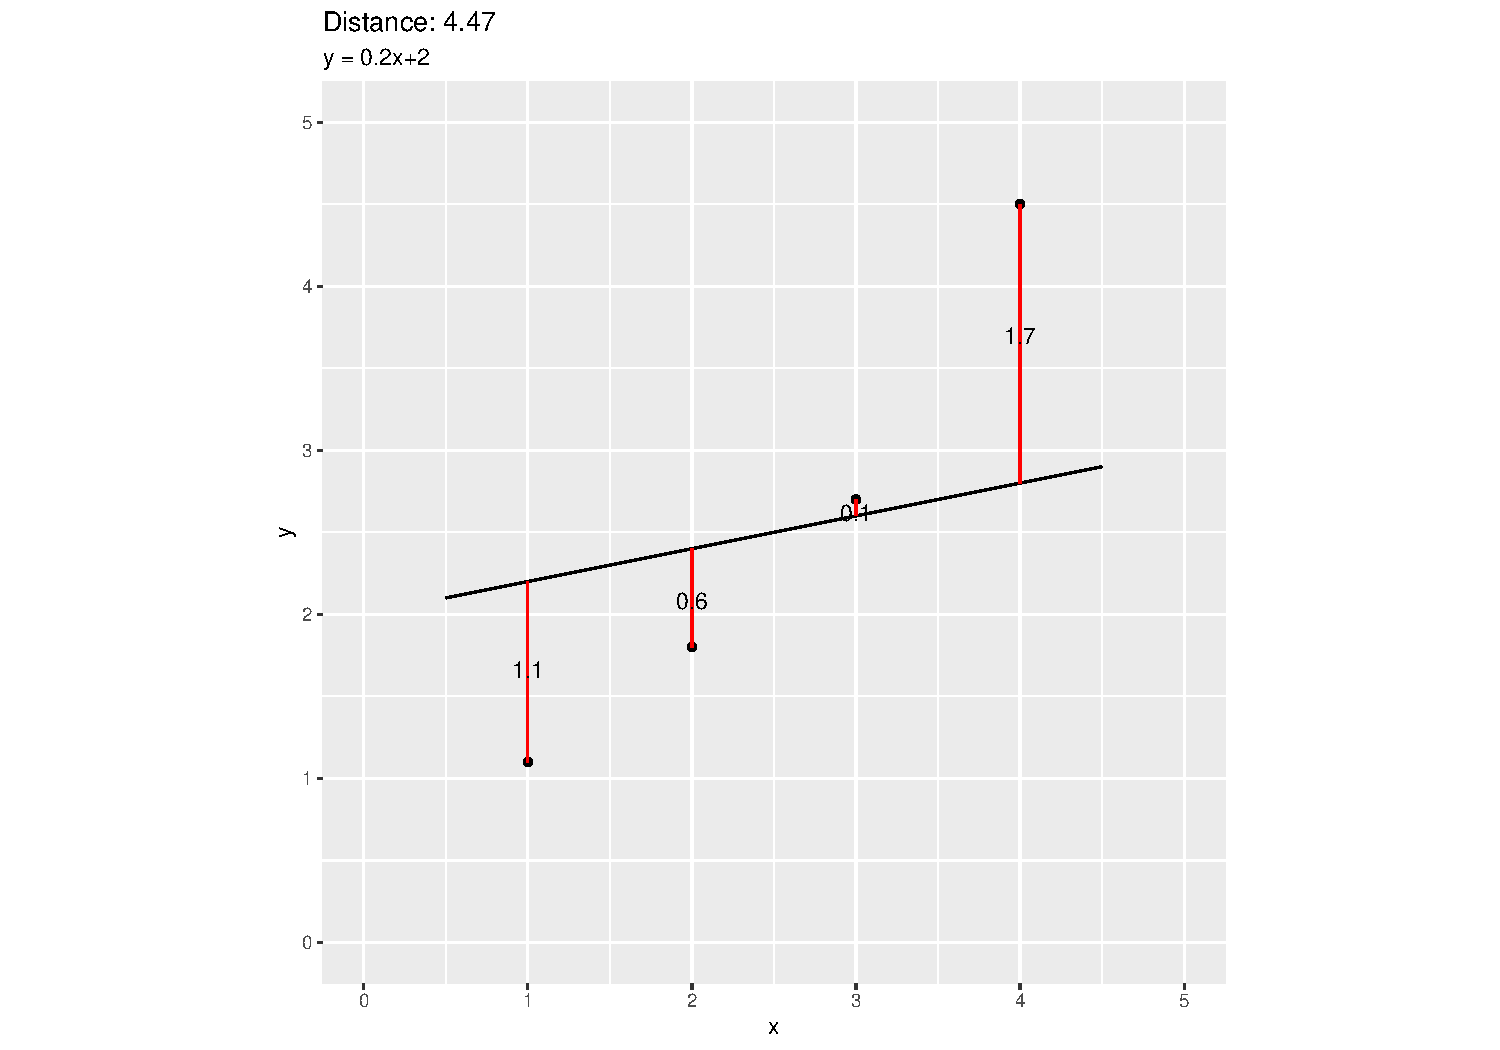
\includegraphics{1_files/figure-beamer/unnamed-chunk-11-1.pdf}
\end{frame}

\begin{frame}{Some other lines}
\protect\hypertarget{some-other-lines-3}{}
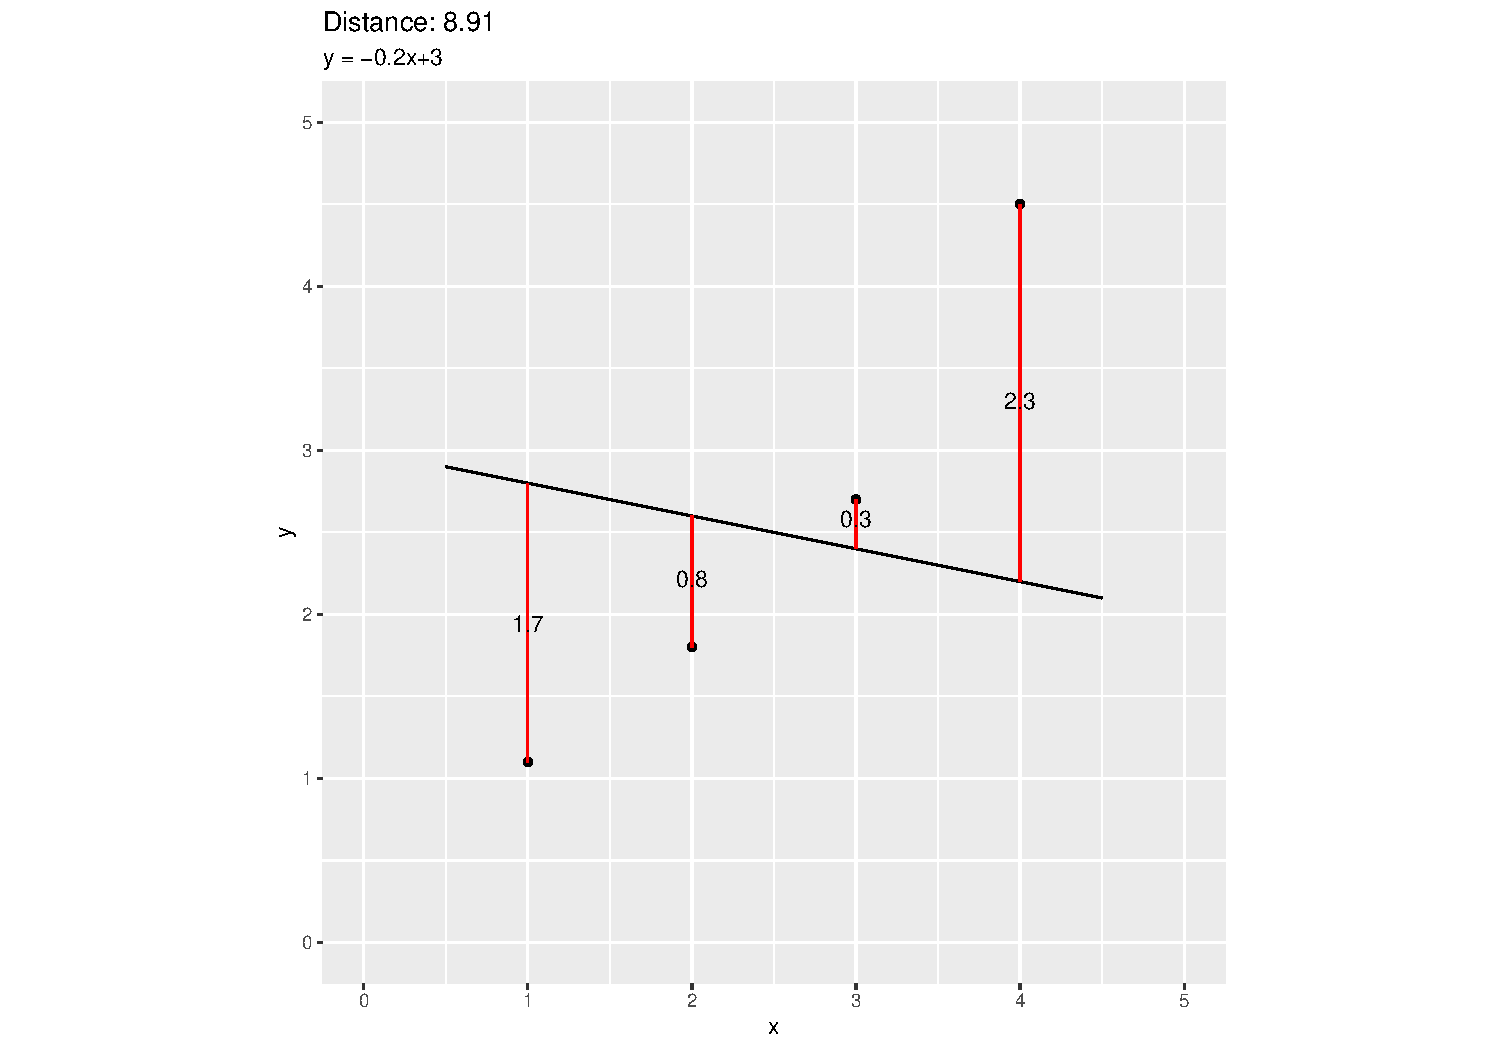
\includegraphics{1_files/figure-beamer/unnamed-chunk-12-1.pdf}
\end{frame}

\begin{frame}{Sum Up}
\protect\hypertarget{sum-up}{}
\begin{itemize}
\tightlist
\item
  The best fitted line or the least squared line is the line that is
  closet to the data point in term of the squared distance.
\end{itemize}
\end{frame}



\end{document}
